% Project Solution Approach 
\section{Project Solution Approach}
Working in a big team with tight deadlines was one of the challenges. Work distribution based on individuals expertise was important. Our team started with project team discussion which focused on following:

\begin{itemize}
	\item Project story discussion
	\item Project story verification analysis
	\item Various technologies involved
	\item Solution designing steps
	\item Work distributions as per expertise
\end{itemize}

\par
\noindent We have used various tools to facilitate our project work:
% \begin{itemize}
% 	\item Github repository 
% 	\item Github project management
% 	\item Overleaf latex Account
% \end{itemize}

\subsection{Github Repository}
We have worked on a private git repo \url{https://github.com/abhinavcreed13/ProjectSDS} with multiple branches. Everyone in the team worked on an independent branch. Once the module was finished, we merged it with the master branch.  

\subsection{Project Management}
We have used several features of Github for managing the entire cycle of this project. Using these features, we are able to work on the issues and discuss enhancements very efficiently.

\texttt{Branches.} We have created separate branch for each user who is working on their individual modules and section of the project. We have distributed our work with the focus of avoiding conflicts and merge issues. With this approach, our \texttt{master} branch remains clean and only stable and tested code is pushed to the branch.

\texttt{Issues.} We have used issues feature of github for allocating required enhancements and development to the respective teammates. This feature helped us to track the progress of the project in a very efficient manner.

\begin{figure}[H]
  \centering%
    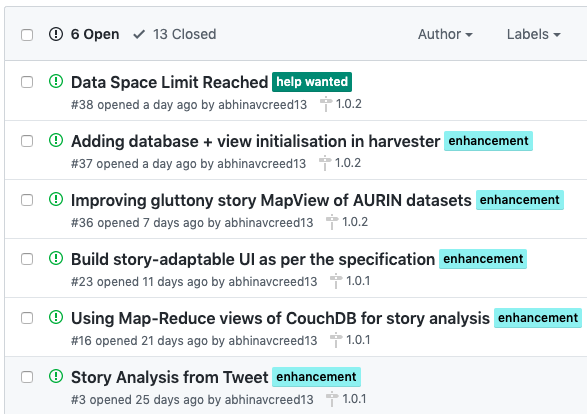
\includegraphics[width=.45\linewidth]{images/git/open_issues.png}\hfill%
    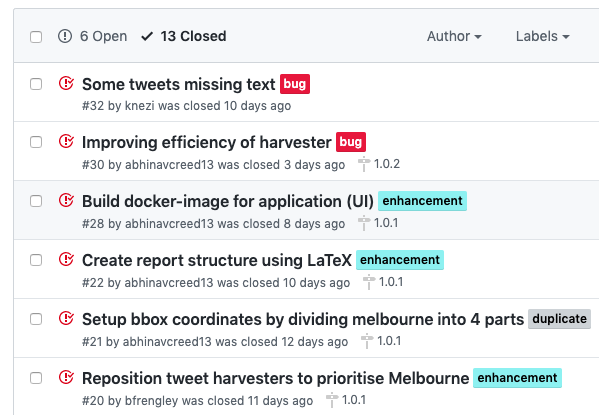
\includegraphics[width=.45\linewidth]{images/git/closed_issues.png}%
    \caption{Task Management using issues}
\end{figure}

\texttt{Project Board.} We have also used project boards to streamline our process by moving and managing items with pipelines. We have also included pull requests in this \texttt{kanban board} to view and see how our project is progressing through various stages.

\begin{figure}[H]
    \centering
    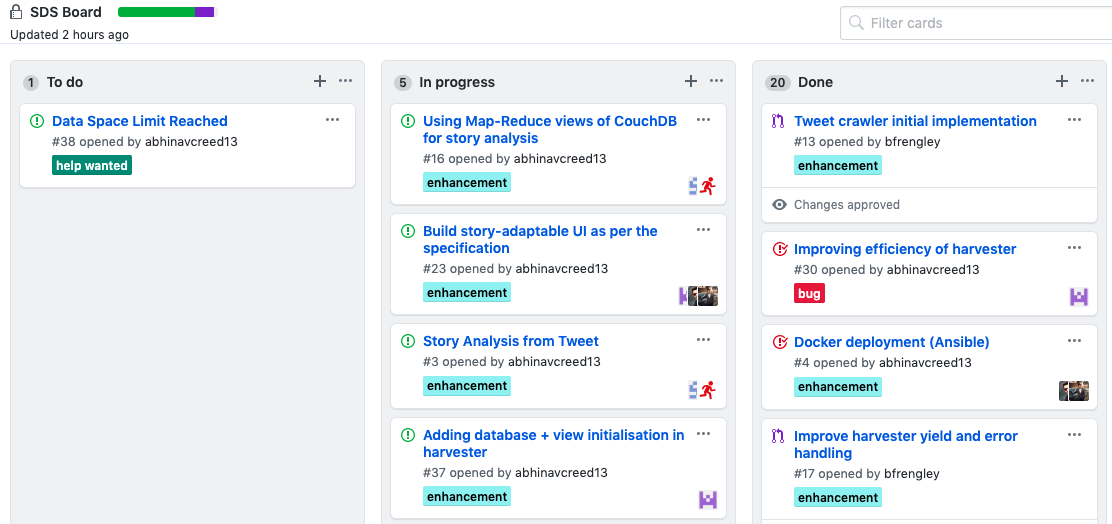
\includegraphics[width=15cm,keepaspectratio=true]{images/git/board_github.png}
    \caption{Managing project pipeline using boards}
\end{figure}

\texttt{Milestones.} With the help of this feature, we analyzed the growth of our project. We tagged our project's progress using milestones which also helped us to group issues on the basis of their versions.

\begin{figure}[H]
    \centering
    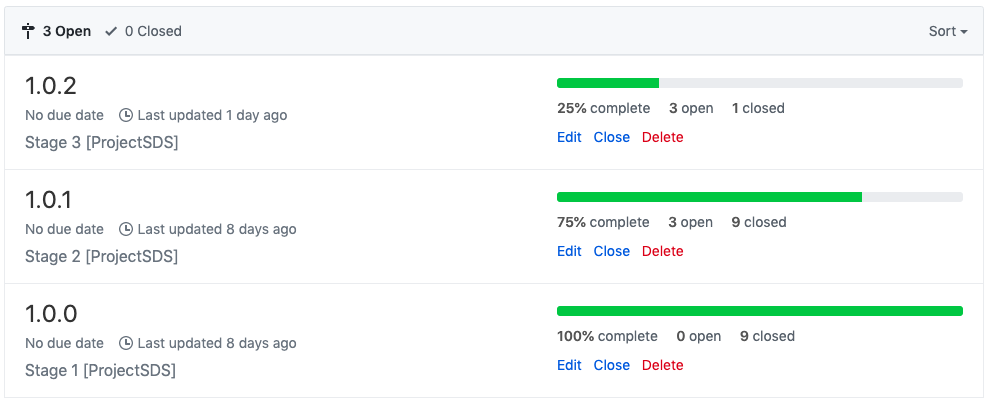
\includegraphics[width=12cm,keepaspectratio=true]{images/git/git_milestones.png}
    \caption{Analyzing progress using milestones}
\end{figure}

\import{}{roles.tex}
%\subsection{Overleaf LaTeX Account}
%\import{content/rohit/}{latex.tex}

